\documentclass[conference,10pt]{IEEEtran}
\IEEEoverridecommandlockouts

\usepackage[T1]{fontenc}
\usepackage{amsmath,amssymb}
\usepackage{graphicx}
\usepackage{booktabs,tabularx,array,multirow}
\usepackage[table]{xcolor}
\usepackage{cite}
\usepackage[expansion=false]{microtype}
\usepackage{tikz}
\usepackage[hidelinks]{hyperref}
\usepackage{url}
\usepackage{balance}
% Shared TikZ look for every diagram in the report: soft fills, rounded corners,
% blurred drop shadows, one sans-serif face — a clean "diagram tool" finish.
\usetikzlibrary{arrows.meta,shadows.blur,shapes.geometric,shapes.symbols,fit,backgrounds,positioning,calc}

\definecolor{inkD}{HTML}{1F2937}
\definecolor{inkM}{HTML}{4B5563}
\definecolor{inkL}{HTML}{6B7280}
\definecolor{appF}{HTML}{EEF2FF}\definecolor{appS}{HTML}{4F46E5}
\definecolor{modF}{HTML}{FFFFFF}\definecolor{modS}{HTML}{818CF8}
\definecolor{dbF}{HTML}{ECFDF5}\definecolor{dbS}{HTML}{059669}
\definecolor{wkF}{HTML}{F5F3FF}\definecolor{wkS}{HTML}{7C3AED}
\definecolor{exF}{HTML}{FFF7ED}\definecolor{exS}{HTML}{EA580C}
\definecolor{uiF}{HTML}{F0F9FF}\definecolor{uiS}{HTML}{0284C7}
\definecolor{secF}{HTML}{FEF2F2}\definecolor{secS}{HTML}{DC2626}
\definecolor{bndS}{HTML}{94A3B8}
\definecolor{flow}{HTML}{475569}

\tikzset{
  font=\sffamily\scriptsize, >={Stealth[length=2.2mm,width=1.6mm]},
  card/.style={rounded corners=2.5pt, line width=0.6pt, align=center, inner sep=4pt,
               blur shadow={shadow blur steps=6, shadow xshift=0.35mm, shadow yshift=-0.45mm, shadow opacity=22}},
  app/.style={card, draw=appS, fill=appF},
  mod/.style={card, draw=modS, fill=modF, minimum width=2.55cm, minimum height=1.02cm, text width=2.4cm},
  ext/.style={card, draw=exS, fill=exF, minimum width=3.0cm, minimum height=1.25cm, text width=2.85cm},
  ui/.style={card, draw=uiS, fill=uiF, minimum width=3.0cm, minimum height=1.25cm, text width=2.85cm},
  wk/.style={card, draw=wkS, fill=wkF, minimum width=2.75cm, minimum height=1.15cm, text width=2.6cm},
  sec/.style={card, draw=secS, fill=secF, minimum height=0.55cm},
  db/.style={cylinder, shape border rotate=90, aspect=0.16, draw=dbS, fill=dbF, line width=0.6pt, align=center,
             blur shadow={shadow blur steps=6, shadow xshift=0.35mm, shadow yshift=-0.45mm, shadow opacity=22}},
  ttl/.style={font=\sffamily\bfseries\scriptsize, text=inkD},
  sub/.style={font=\sffamily\tiny, text=inkM},
  lbl/.style={font=\sffamily\tiny, text=inkM, fill=white, fill opacity=0.92, text opacity=1, inner sep=1.2pt, rounded corners=1pt},
  arr/.style={->, draw=flow, line width=0.75pt, rounded corners=3pt},
  arr2/.style={<->, draw=flow, line width=0.75pt, rounded corners=3pt},
  rdash/.style={->, draw=flow, line width=0.7pt, dashed, dash pattern=on 2.5pt off 1.5pt, rounded corners=3pt},
  boundary/.style={draw=bndS, line width=0.8pt, dash pattern=on 4pt off 2.5pt, rounded corners=6pt},
  zonelbl/.style={font=\sffamily\bfseries\tiny, text=inkL, fill=white, inner sep=2pt},
  badge/.style={circle, fill=#1, text=white, font=\sffamily\bfseries\tiny, inner sep=0.8pt, minimum size=3.4mm},
}

% A small person glyph: \person{name}{x,y}{label}
\newcommand{\person}[3]{%
  \begin{scope}[shift={(#2)}]
    \fill[uiS!85] (0,0.26) circle (0.11);
    \fill[uiS!85] (-0.19,-0.02) .. controls (-0.19,0.14) and (0.19,0.14) .. (0.19,-0.02) -- cycle;
    \node[sub, anchor=north] (#1) at (0,-0.04) {#3};
  \end{scope}}


\newcolumntype{L}{>{\raggedright\arraybackslash}X}
\newcommand{\tbl}{\scriptsize\renewcommand{\arraystretch}{1.12}}
\newcommand{\code}[1]{\texttt{\small #1}}
% Test names: monospace, allowed to break after underscores.
\makeatletter\g@addto@macro{\UrlBreaks}{\do\_}\makeatother
\DeclareUrlCommand\tn{\urlstyle{tt}}
% Generated by scripts/export_results.py — do not edit.
\newcommand{\ResTxns}{57,055}
\newcommand{\ResDays}{29}
\newcommand{\ResAlerts}{468}
\newcommand{\ResIllicitPct}{0.61\%}
\newcommand{\ResAccountsAlerted}{192}
\newcommand{\ResTP}{47}
\newcommand{\ResIllicitActive}{56}
\newcommand{\ResPrecisionPct}{24\%}
\newcommand{\ResRecallPct}{84\%}
\newcommand{\ResMLPRAUC}{0.89}
\newcommand{\ResMLROC}{0.999}
\newcommand{\ResMLPrec}{0.79}
\newcommand{\ResMLRec}{0.83}
\newcommand{\ResMLTestTxns}{117,249}
\newcommand{\ResMLTestIllicit}{349}
\newcommand{\ResMLCommittee}{6\%}
\newcommand{\ResTests}{38}


\begin{document}

\title{WalletWatch: An Assured, Near-Real-Time\\Anti-Money-Laundering Monitoring System\\for Mobile Wallets}

\author{\IEEEauthorblockN{Hafiz Farhad Ahmed (22K-4787)}
\IEEEauthorblockA{Information Assurance --- Course Project\\
Department of Computer Science, FAST-NUCES Karachi\\
Instructor: Ali Naseer}}

\maketitle

\begin{abstract}
Mobile wallets make it cheap and instant to move money, and so make it easy to launder.
Regulators require wallet operators to monitor transactions and report suspicious activity, but
the monitoring system is itself a high-value target: it holds identity data, decides who is
investigated and produces legal reports. We present \emph{WalletWatch}, a working, containerised
anti-money-laundering (AML) monitoring system for a synthetic Pakistani mobile wallet. It
combines typology rules, a temporal graph search and an explained gradient-boosted model, and wraps
them in an analyst workflow built on Information Assurance (IA) principles: least privilege,
role-based access control, maker--checker separation of duties, personal-data masking and a
keyed, tamper-evident audit log. We assess the system against ISO/IEC~27001:2022, NIST SP~800-53
Rev.~5 and the NIST Cybersecurity Framework~2.0, perform an ISO~31000 / NIST SP~800-30 risk
assessment including cyber-insurance as a risk-transfer option, and design a Security Education,
Training and Awareness (SETA) programme for its users. On a held-out synthetic world the model
reaches a PR-AUC of \ResMLPRAUC; in a \ResDays-day live run the full system detects
\ResRecallPct\ of active laundering accounts at an account-level precision of \ResPrecisionPct,
and every IA control is verified by an automated test.
\end{abstract}

\begin{IEEEkeywords}
anti-money laundering, transaction monitoring, information assurance, separation of duties,
tamper-evident logging, risk management, ISO/IEC 27001, NIST, SETA, cyber insurance
\end{IEEEkeywords}

% =====================================================================================
\section{Introduction}

Money laundering is classically described in three stages: \emph{placement} of criminal proceeds
into the financial system, \emph{layering} to obscure their origin, and \emph{integration} back into
the legitimate economy~\cite{fatf2012rec}. Mobile money serves all three. Cash enters through a
dense network of agents, transfers between wallets are instant and cheap, and low-value accounts can
be opened with light identification~\cite{fatf2013npps,gsma2015proportional}. Pakistan's
Anti-Money Laundering Act 2010 therefore obliges reporting entities to file Suspicious Transaction
Reports (STRs) and Currency Transaction Reports (CTRs) with the Financial Monitoring Unit (FMU)
through its goAML platform~\cite{amla2010,fmu2021ctr,nibaf2026goaml}.

Two problems make this hard in practice. The first is detection quality: rule-based monitoring is
explainable but noisy, with industry reports of false-positive rates well above
90\%~\cite{deloitte2020tm}. The second, central to this course, is that the monitoring system is a
security-critical asset. It stores national identity numbers (CNICs) and phone numbers, its
decisions determine which customers are investigated, and its output is a legal report. An insider
who can silence an alert, approve their own report or rewrite the audit trail defeats the purpose
of the system.

\textbf{Contributions.} This project delivers:
\begin{itemize}
  \item a synthetic Pakistani wallet with ten planted laundering rings and \emph{benign look-alike}
        behaviour (committees, salary runs, family remittances, shared phones), so that the
        evaluation measures honest false positives rather than a circular fit;
  \item a near-real-time detection pipeline of six typologies, combining rules, a temporal graph
        search, and an XGBoost model explained per transaction with SHAP;
  \item a secured analyst workflow (alert $\rightarrow$ case $\rightarrow$ STR) with role-based
        access control, maker--checker approval enforced in two layers, PII masking and an
        HMAC-keyed, hash-chained audit log;
  \item an IA assessment: an assurance case with test evidence, a standards mapping (ISO/IEC 27001,
        NIST SP 800-53, CSF 2.0, FATF), an ISO 31000 risk register with treatment including cyber
        insurance, and a SETA programme.
\end{itemize}

% =====================================================================================
\section{Background and Literature Review}

\subsection{Laundering through mobile money}
FATF guidance identifies the agent network, multiple accounts per person and rapid
person-to-person transfers as the main risk factors in mobile payments~\cite{fatf2013npps}.
Professional laundering relies on networks of money mules that receive and forward funds on
behalf of others~\cite{fatf2018pml}. In Pakistan, branchless-banking wallets are tiered by the depth
of know-your-customer checks, each tier carrying daily, monthly and balance
limits~\cite{sbp2016bb}. Staying just under these limits, or spreading deposits across several
wallets, is the wallet form of \emph{structuring}. Since November 2026 the CTR threshold for
cash transactions is PKR~3 million~\cite{sbp2026cl24}, a value few wallets reach, which places the
burden of detection on STR-style behavioural monitoring.

\subsection{Detection approaches}
Chen et al.~\cite{chen2018amlreview} survey AML detection and find that deployed systems remain
predominantly rule-based, with machine learning applied to scoring, clustering and alert
prioritisation. Jullum et al.~\cite{jullum2020} train gradient-boosted trees on a bank's historical
alerts and show they can rank cases more usefully than rules alone. Because laundering is a property
of \emph{groups} of accounts, network methods have gained ground: Savage et al.~\cite{savage2016}
learn from features of transaction sub-networks, and Weber et al.~\cite{weber2019gcn} apply graph
convolutional networks to illicit Bitcoin flows. Gradient-boosted trees~\cite{chen2016xgboost}
remain a strong, explainable baseline on tabular features~\cite{altman2023amlworld}.

\subsection{Synthetic data}
Real transaction data with laundering labels is almost never public. Agent-based simulators fill the
gap: PaySim~\cite{lopezrojas2016paysim} models mobile-money fraud, AMLSim~\cite{amlsim} generates
laundering typologies over a bank graph, and AMLworld~\cite{altman2023amlworld} adds realistic
placement, layering and integration with perfect labels. WalletWatch follows the same method, adapted
to Pakistani wallet tiers, agents and local benign behaviour.

\subsection{Explainability}
AML decisions must be defensible to regulators and to the customers concerned. SHAP attributes a
prediction additively to its features using Shapley values~\cite{lundberg2017shap}, and TreeSHAP
computes them exactly and efficiently for tree ensembles~\cite{lundberg2020tree}.

\subsection{Securing the monitoring system}
Clark and Wilson argued that commercial integrity rests on well-formed transactions and
\emph{separation of duty}~\cite{clarkwilson1987}, the basis of the maker--checker rule.
Role-based access control~\cite{sandhu1996rbac} maps job functions to permissions. For audit logs,
Haber and Stornetta's hash-linked time-stamping~\cite{haber1991timestamp} and Schneier and Kelsey's
keyed secure audit logs~\cite{schneier1999audit} show how to make tampering detectable even by an
attacker who controls the storage. NIST SP 800-92 gives operational guidance on log
management~\cite{nist80092}.

\subsection{Gap}
The detection literature rarely addresses the security of the system that runs the detection,
while security frameworks are seldom shown applied end to end on a concrete AML system. This project
joins the two: a working detector whose assurance claims are each backed by an automated test.

% =====================================================================================
\section{Requirements and Scope}

\textbf{Functional.} Ingest a stream of wallet transactions; detect structuring, mule fan-in/out,
pass-through, layering and round-tripping, and shared devices; group alerts into cases; let analysts
close or escalate cases with reasons; draft STRs and require approval by a Money Laundering
Reporting Officer (MLRO); measure detection quality against ground truth.

\textbf{Security.} (S1) Only authenticated users act, and only within their role. (S2) No single
person can both draft and approve an STR. (S3) Personal identifiers are hidden unless a justified,
logged request is made. (S4) Every security-relevant action is recorded in a log whose tampering is
detectable. (S5) The detector cannot read the ground truth it is graded on. (S6) Each component
holds the least privilege it needs.

\textbf{Out of scope.} Customer-side fraud (account takeover, SIM swap), sanctions screening,
goAML XML submission, TLS and single sign-on, and real customer data.

% =====================================================================================
\section{System Architecture}\label{sec:arch}

\begin{figure*}[t]
  \centering
  \resizebox{\textwidth}{!}{% System architecture (Fig. 1). Coordinates in cm; scaled to \textwidth by the caller.
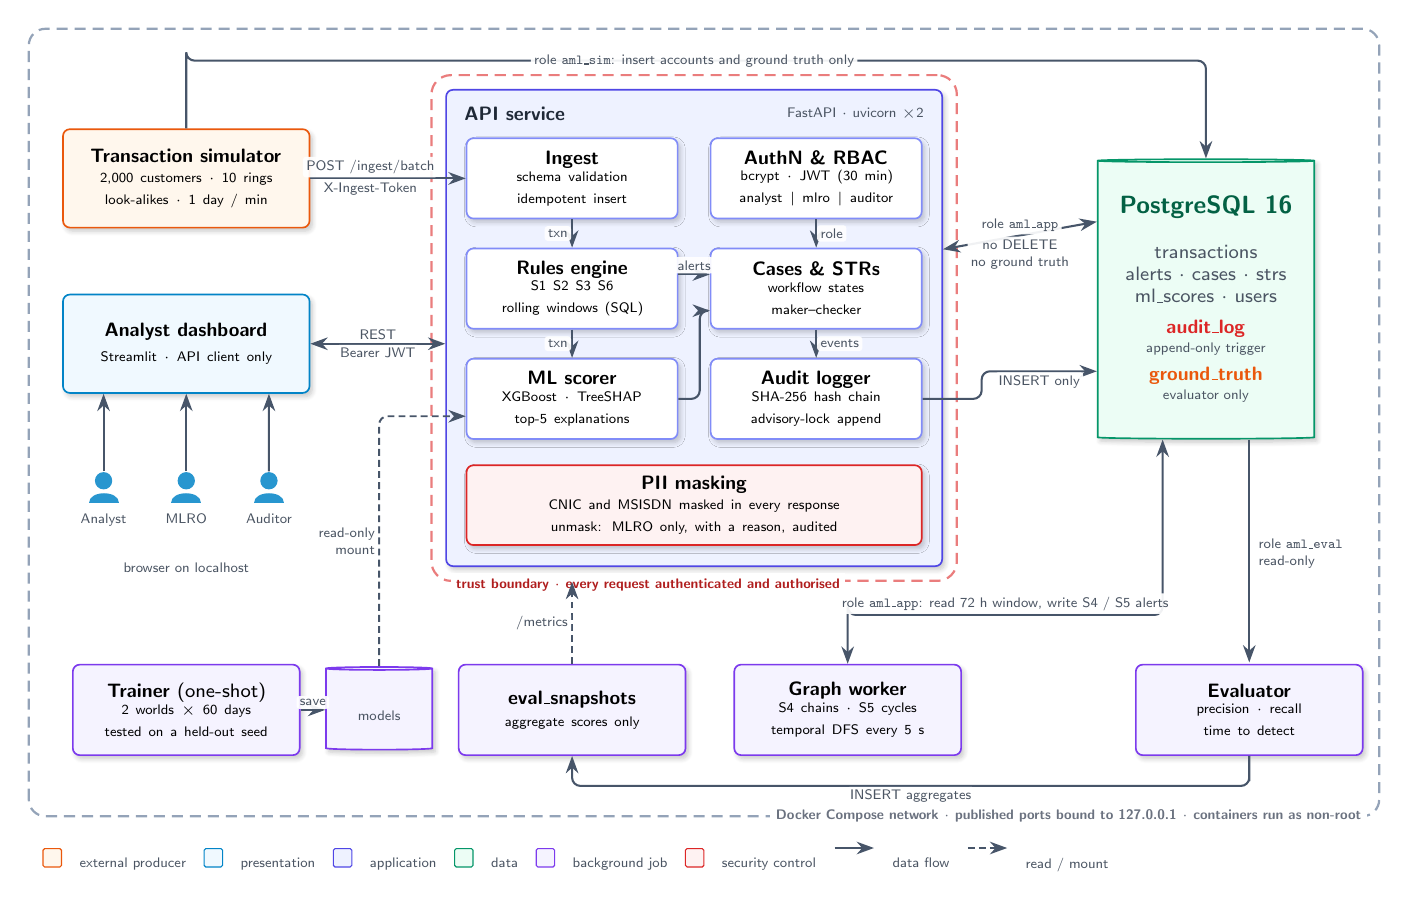
\begin{tikzpicture}[x=1cm,y=1cm]

% ---------------------------------------------------------------- producers and users
\node[ext] (sim)  at (1.6,5.15) {\textbf{Transaction simulator}\\[1pt]{\tiny 2,000 customers $\cdot$ 10 rings\\look-alikes $\cdot$ 1 day / min}};
\node[ui]  (dash) at (1.6,3.05) {\textbf{Analyst dashboard}\\[1pt]{\tiny Streamlit $\cdot$ API client only}};
\person{pA}{0.55,1.05}{Analyst}
\person{pM}{1.6,1.05}{MLRO}
\person{pU}{2.65,1.05}{Auditor}
\foreach \p/\dx in {pA/-1.05, pM/0, pU/1.05}
  \draw[arr] ($(\p.north)+(0,0.42)$) -- ($(dash.south)+(\dx,0)$);
\node[sub] at (1.6,0.2) {browser on localhost};

% ---------------------------------------------------------------- API service
\node[app, minimum width=6.3cm, minimum height=6.05cm] (api) at (8.05,3.25) {};
\node[ttl, anchor=north west] at ($(api.north west)+(0.12,-0.1)$) {API service};
\node[sub, anchor=north east] at ($(api.north east)+(-0.12,-0.12)$) {FastAPI $\cdot$ uvicorn $\times$2};

\node[mod] (ing)  at (6.5,5.15) {\textbf{Ingest}\\{\tiny schema validation\\idempotent insert}};
\node[mod] (auth) at (9.6,5.15) {\textbf{AuthN \& RBAC}\\{\tiny bcrypt $\cdot$ JWT (30 min)\\analyst $\mid$ mlro $\mid$ auditor}};
\node[mod] (rul)  at (6.5,3.75) {\textbf{Rules engine}\\{\tiny S1 S2 S3 S6\\rolling windows (SQL)}};
\node[mod] (case) at (9.6,3.75) {\textbf{Cases \& STRs}\\{\tiny workflow states\\maker--checker}};
\node[mod] (ml)   at (6.5,2.35) {\textbf{ML scorer}\\{\tiny XGBoost $\cdot$ TreeSHAP\\top-5 explanations}};
\node[mod] (aud)  at (9.6,2.35) {\textbf{Audit logger}\\{\tiny SHA-256 hash chain\\advisory-lock append}};
\node[sec, minimum width=5.65cm, text width=5.5cm] (mask) at (8.05,1.0)
      {\textbf{PII masking}\\[1pt]{\tiny CNIC and MSISDN masked in every response\\ unmask: MLRO only, with a reason, audited}};

\draw[arr] (ing) -- node[lbl, left] {txn} (rul);
\draw[arr] (rul) -- node[lbl, left] {txn} (ml);
\draw[arr] ($(rul.east)+(0,0.18)$) -- node[lbl, above] {alerts} ($(case.west)+(0,0.18)$);
\draw[arr] (ml.east) -- ++(0.27,0) |- ($(case.west)+(0,-0.28)$);
\draw[arr] (case) -- node[lbl, right] {events} (aud);
\draw[arr] (auth) -- node[lbl, right] {role} (case);

\node[fit=(api), inner sep=5pt, draw=secS!60, line width=0.8pt, dash pattern=on 4pt off 2.5pt, rounded corners=7pt] (tb) {};
\node[zonelbl, text=secS!80!black, anchor=north west] at ($(tb.south west)+(0.25,0.12)$) {trust boundary $\cdot$ every request authenticated and authorised};

% ---------------------------------------------------------------- data tier
\node[db, minimum width=2.75cm, minimum height=3.55cm] (pg) at (14.55,3.6) {};
\node[ttl, text=dbS!65!black, font=\sffamily\bfseries\small] at ($(pg.north)+(0,-0.62)$) {PostgreSQL 16};
\node[font=\sffamily\scriptsize, text=inkM, align=center, anchor=north] at ($(pg.north)+(0,-0.98)$) {%
  transactions\\ alerts $\cdot$ cases $\cdot$ strs\\ ml\_scores $\cdot$ users\\[3pt]
  {\color{secS}\textbf{audit\_log}}\\[-1pt]{\tiny append-only trigger}\\[2pt]
  {\color{exS}\textbf{ground\_truth}}\\[-1pt]{\tiny evaluator only}};

% ---------------------------------------------------------------- background jobs
\node[wk] (tr)   at (1.6,-1.6)   {\textbf{Trainer} (one-shot)\\{\tiny 2 worlds $\times$ 60 days\\tested on a held-out seed}};
\node[db, minimum width=1.35cm, minimum height=1.05cm, draw=wkS, fill=wkF] (vol) at (4.05,-1.6) {};
\node[sub] at ($(vol.center)+(0,-0.07)$) {models};
\node[wk] (snap) at (6.5,-1.6)   {\textbf{eval\_snapshots}\\{\tiny aggregate scores only}};
\node[wk] (gw)   at (10.0,-1.6)  {\textbf{Graph worker}\\{\tiny S4 chains $\cdot$ S5 cycles\\temporal DFS every 5 s}};
\node[wk] (ev)   at (15.1,-1.6)  {\textbf{Evaluator}\\{\tiny precision $\cdot$ recall\\time to detect}};

% ---------------------------------------------------------------- flows between tiers
\draw[arr] (sim.east) -- node[lbl, above] {POST /ingest/batch} node[lbl, below] {X-Ingest-Token} (sim.east -| tb.west) -- (ing.west);
\draw[arr] (sim.north) |- ++(0,0.86) -| (pg.north);
\node[lbl] at (8.05,6.64) {role \texttt{aml\_sim}: insert accounts and ground truth only};
\draw[arr2] (dash.east) -- node[lbl, above] {REST} node[lbl, below] {Bearer JWT} (dash.east -| api.west);
\draw[arr2] ($(api.east)+(0,1.0)$) -- node[lbl, above] {role \texttt{aml\_app}} node[lbl, below, align=center] {no DELETE\\no ground truth} ($(pg.west)+(0,1.0)$);
\draw[arr] (aud.east) -- ++(0.75,0) |- node[lbl, pos=0.75, below] {INSERT only} ($(pg.west)+(0,-0.9)$);
\draw[arr2] (gw.north) |- ++(0,0.62) -| node[lbl, pos=0.25, above] {role \texttt{aml\_app}: read 72 h window, write S4 / S5 alerts} ($(pg.south)+(-0.55,0)$);
\draw[arr] ($(pg.south)+(0.55,0)$) -- ($(pg.south)+(0.55,-2.83)$);
\node[lbl, anchor=west, align=left] at ($(pg.south)+(0.62,-1.45)$) {role \texttt{aml\_eval}\\read-only};
\draw[arr] (ev.south) |- ++(0,-0.38) -| node[lbl, pos=0.25, below] {INSERT aggregates} (snap.south);
\draw[rdash] (snap.north) -- node[lbl, left] {/metrics} (snap.north |- tb.south);
\draw[arr] (tr.east) -- node[lbl, above] {save} (vol.west);
\draw[rdash] (vol.north) |- node[lbl, pos=0.25, left, align=right] {read-only\\mount} ($(ml.south west)+(0,0.3)$);

% ---------------------------------------------------------------- outer boundary + legend
\begin{scope}[on background layer]
  \draw[boundary] (-0.4,-2.95) rectangle (16.75,7.05);
\end{scope}
\node[zonelbl, anchor=east] at (16.6,-2.95) {Docker Compose network $\cdot$ published ports bound to 127.0.0.1 $\cdot$ containers run as non-root};

\matrix[anchor=north west, column sep=3pt, font=\sffamily\tiny, text=inkM] at (-0.35,-3.15) {
  \node[fill=exF, draw=exS, minimum size=2.2mm, rounded corners=0.6pt]{}; & \node{external producer}; &
  \node[fill=uiF, draw=uiS, minimum size=2.2mm, rounded corners=0.6pt]{}; & \node{presentation}; &
  \node[fill=appF, draw=appS, minimum size=2.2mm, rounded corners=0.6pt]{}; & \node{application}; &
  \node[fill=dbF, draw=dbS, minimum size=2.2mm, rounded corners=0.6pt]{}; & \node{data}; &
  \node[fill=wkF, draw=wkS, minimum size=2.2mm, rounded corners=0.6pt]{}; & \node{background job}; &
  \node[fill=secF, draw=secS, minimum size=2.2mm, rounded corners=0.6pt]{}; & \node{security control}; &
  \draw[arr] (0,0) -- (0.5,0); & \node{data flow}; &
  \draw[rdash] (0,0) -- (0.5,0); & \node{read / mount}; \\
};
\end{tikzpicture}
}
  \caption{WalletWatch architecture. Every service runs in one Docker Compose network with published
  ports bound to localhost. The API is the single trust boundary for people. Each container connects
  to PostgreSQL under its own least-privilege role, and the API alone holds the audit-chain key.}
  \label{fig:arch}
\end{figure*}

Fig.~\ref{fig:arch} shows the deployment: six containers, started with one command.

\textbf{Simulator.} It generates the synthetic world (Section~\ref{sec:world}) and streams it to
the API at a configurable speed (by default one simulated day per real minute), authenticating with a
dedicated ingest token. It writes accounts and ground truth directly, but only through the
\code{aml\_sim} role, which may insert into those tables and nothing else.

\textbf{API service.} A FastAPI application is the only component people interact with. Per
transaction it validates the input schema, inserts idempotently (the transaction id is the primary
key), evaluates the rules, scores the model and creates alerts, all within one database
transaction. It also implements authentication, RBAC, case and STR workflows, PII masking and the
audit logger.

\textbf{Graph worker.} Every five seconds it loads the recent customer-to-customer transfer graph
and searches for time-ordered chains and cycles (S4, S5).

\textbf{Dashboard.} A Streamlit interface for the three roles. It holds only a short-lived JWT and
never connects to the database, so all enforcement happens behind the API.

\textbf{Evaluator.} It runs as the read-only \code{aml\_eval} role, joins alerts with ground truth
and writes \emph{aggregate} scores to \code{eval\_snapshots}. The API can read those aggregates but
never the per-account answers (requirement S5).

\textbf{Trainer.} A one-shot job that trains the model into a volume mounted read-only into the API.

\begin{table}[t]
\caption{Database roles (least privilege, requirement S6)}\label{tab:roles}
\centering\tbl
\begin{tabularx}{\columnwidth}{@{}lL@{}}
\toprule
Role & Privileges \\ \midrule
\code{aml\_app}  & SELECT/INSERT/UPDATE on operational tables; INSERT-only on \code{audit\_log}; no DELETE anywhere; no access to \code{ground\_truth} \\
\code{aml\_sim}  & INSERT accounts and ground truth only \\
\code{aml\_eval} & SELECT everything; INSERT into \code{eval\_snapshots} only \\
\code{postgres}  & initialisation only; password never given to application containers \\
\bottomrule
\end{tabularx}
\end{table}

% =====================================================================================
\section{Detection Design}\label{sec:world}

\subsection{Synthetic world}
The simulator creates 2,000 customers in twelve cities with CNICs, phone numbers, devices and
wallet tiers L0/L1/L2, together with 50 cash agents, 20 billers, five employers and five external
banks. Normal behaviour includes top-ups, bills, transfers to a stable set of contacts, and cash-in
and cash-out at a home agent, with a daily cycle and an Eid spending spike. Ten laundering rings,
two per typology, are recruited from ordinary customers, so account identifiers and profiles reveal
nothing. Benign look-alikes deliberately resemble laundering: \emph{committees} (rotating savings
groups whose members pay one organiser), salary fan-outs, family remittance chains, and households
sharing one phone. Illicit transactions make up \ResIllicitPct\ of the live run.

\subsection{Typologies}
Table~\ref{tab:typ} lists the scenarios. All thresholds live in one configuration file, and every
window is evaluated in simulated time.

\begin{table}[t]
\caption{Detection scenarios}\label{tab:typ}
\centering\tbl
\begin{tabularx}{\columnwidth}{@{}llL@{}}
\toprule
ID & Typology & Fires when \\ \midrule
S1 & Structuring & $\geq$3 credits in 7\,d, each 85--100\% of the tier daily limit \\
S2 & Fan-in/out mule & in 24\,h: $\geq$8 senders, $\geq$5 receivers, out $\geq$80\% of in \\
S3 & Pass-through & $\geq$90\% of a credit $\geq$PKR\,20k leaves within 60\,min, twice in 7\,d \\
S4 & Layering chain & $\geq$4 time-ordered hops in 6\,h, each 85--100\% of the previous \\
S5 & Round-trip & return to origin via 3--6 accounts in 72\,h, $\geq$70\% returned \\
S6 & Shared device & $\geq$3 wallets used on one device in 7\,d \\
ML & Model risk & $p \geq 0.80$ on a transaction no rule flagged \\
\bottomrule
\end{tabularx}
\end{table}

\textbf{Temporal graph search.} A standard cycle algorithm would report a ``round-trip'' even when
the money moved backwards in time. The worker instead runs a depth-first search in which each hop
must occur after the previous one and within the window. Chains are reported only from their
\emph{head}, the first hop with no qualifying predecessor, so a chain that grows between ticks
keeps a single identity and is not alerted twice.

\textbf{Model.} Twenty-four features describe each transaction: its amount relative to the tier
limit, the sender's and receiver's counterparty counts over 24\,h, whether the pair has transacted
before, minutes since the sender's last credit, the share forwarded within the hour, and the number of
wallets seen on the device. One feature function serves both training (an in-memory replay) and
live scoring (history fetched from PostgreSQL), so the two cannot drift apart. XGBoost is trained
on two 60-day worlds and tested on a third with a different seed. Every live score stores its five
largest TreeSHAP contributions.

\textbf{Alerts as evidence.} An alert freezes the transactions and the numbers that crossed the
threshold, and stores the SHA-256 of their canonical JSON. The case view recomputes the hash on
every read and flags any mismatch.

% =====================================================================================
\section{Analyst Workflow and Separation of Duties}

\begin{figure}[t]
  \centering
  \resizebox{\columnwidth}{!}{% Case lifecycle with maker-checker (Fig. 2). Single-column width.
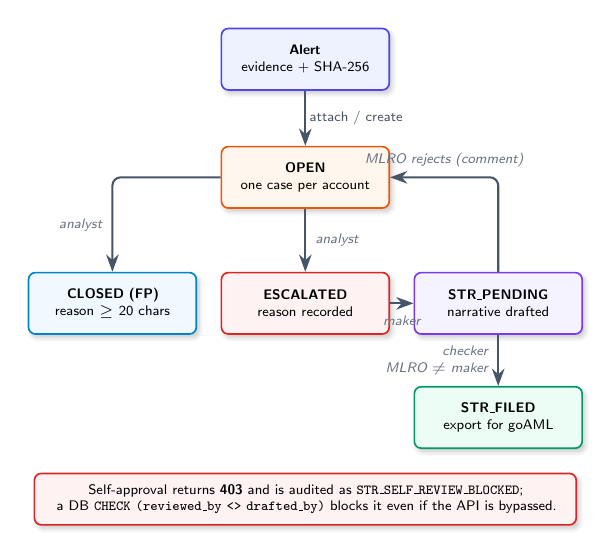
\begin{tikzpicture}[x=1cm,y=1cm,
  st/.style={card, minimum width=1.95cm, minimum height=0.78cm, text width=1.85cm, font=\sffamily\tiny},
  open/.style={st, draw=exS, fill=exF}, esc/.style={st, draw=secS, fill=secF},
  pend/.style={st, draw=wkS, fill=wkF}, done/.style={st, draw=dbS, fill=dbF}, fp/.style={st, draw=uiS, fill=uiF},
  who/.style={font=\sffamily\tiny\itshape, text=inkL}]

\node[st, draw=appS, fill=appF] (al) at (0,2.2)   {\textbf{Alert}\\evidence + SHA-256};
\node[open] (op) at (0,0.7)  {\textbf{OPEN}\\one case per account};
\node[fp]   (fp) at (-2.45,-0.9) {\textbf{CLOSED (FP)}\\reason $\geq$ 20 chars};
\node[esc]  (es) at (0,-0.9) {\textbf{ESCALATED}\\reason recorded};
\node[pend] (sp) at (2.45,-0.9) {\textbf{STR\_PENDING}\\narrative drafted};
\node[done] (sf) at (2.45,-2.35) {\textbf{STR\_FILED}\\export for goAML};

\draw[arr] (al) -- node[lbl, right] {attach / create} (op);
\draw[arr] (op.west) -| node[who, pos=0.75, left] {analyst} (fp.north);
\draw[arr] (op) -- node[who, right] {analyst} (es);
\draw[arr] (es) -- node[who, below, yshift=-1pt] {maker} (sp);
\draw[arr] (sp) -- node[who, left, align=right] {checker\\MLRO $\neq$ maker} (sf);
\draw[arr] (sp.north) |- node[who, pos=0.75, above] {MLRO rejects (comment)} (op.east);

\node[sec, font=\sffamily\tiny, text width=6.6cm, anchor=north] at (0,-3.05)
  {Self-approval returns \textbf{403} and is audited as \texttt{STR\_SELF\_REVIEW\_BLOCKED};\\
   a DB \texttt{CHECK (reviewed\_by <> drafted\_by)} blocks it even if the API is bypassed.};
\end{tikzpicture}
}
  \caption{Case lifecycle. The analyst is the \emph{maker}, the MLRO the \emph{checker}; the same
  person can never be both for one STR.}
  \label{fig:workflow}
\end{figure}

Alerts on the same account join its single active case, which is enforced by a partial unique
index. Fig.~\ref{fig:workflow} shows the lifecycle. A false-positive closure requires a written
reason of at least 20 characters, enforced by both the API and a database \code{CHECK}. Escalation
lets the analyst draft an STR from a template pre-filled with the evidence. Only an MLRO who did
\emph{not} draft the STR may approve it. A self-approval attempt is refused (HTTP~403) and logged,
and the database rejects it independently through \code{CHECK (reviewed\_by <> drafted\_by)}, so a
bug or bypass in the API cannot violate the rule. A filed STR is exported for submission through
goAML.

% =====================================================================================
\section{Information Assurance Perspective}\label{sec:ia}

\subsection{IA services}
The McCumber cube extended by Maconachy et al.~\cite{maconachy2001msr} frames assurance as
\emph{information states} (storage, processing, transmission) $\times$ \emph{security services}
$\times$ \emph{countermeasures} (technology, policy, people). Table~\ref{tab:pillars} maps the five
IA services to WalletWatch. The people dimension is addressed by the SETA programme in
Section~\ref{sec:seta}.

\begin{table}[t]
\caption{IA services and how WalletWatch provides them}\label{tab:pillars}
\centering\tbl
\begin{tabularx}{\columnwidth}{@{}lL@{}}
\toprule
Service & Mechanisms \\ \midrule
Confidentiality & RBAC on every endpoint; CNIC/MSISDN masked in all responses; audited, justified unmask (MLRO only); ground truth unreadable by the app role \\
Integrity & keyed hash-chained audit log; hashed alert evidence; maker--checker; DB constraints duplicate API rules; no DELETE privilege \\
Availability & health checks and restart policies; idempotent ingest with client retry; stateless API workers \\
Authentication & bcrypt password hashes; 30-min signed JWT; role re-read from the DB on each request; uniform login errors \\
Non-repudiation & every action attributed to an authenticated user in a keyed chain. \emph{Partial}: no per-user digital signatures \\
\bottomrule
\end{tabularx}
\end{table}

\subsection{Assurance case}
Assurance means \emph{justified confidence} that the controls work. Table~\ref{tab:assurance}
states each security claim, the argument for it, and the automated test that is its evidence.
The suite (\ResTests\ tests) runs against the live containers.

\begin{table}[t]
\caption{Assurance case: claims, arguments, evidence}\label{tab:assurance}
\centering\tbl
\begin{tabularx}{\columnwidth}{@{}p{1.85cm}Lp{2.55cm}@{}}
\toprule
Claim & Argument & Evidence (test) \\ \midrule
Only authorised roles act & role checked per request from DB; denial audited & \tn{test_rbac_matrix} \\
Forged tokens fail & HS256 signature, expiry required & \tn{test_no_or_forged_token_rejected} \\
No self-approval & API check + DB \code{CHECK} & \tn{test_case_workflow_and_maker_checker}, \tn{test_maker_checker_constraint} \\
PII hidden by default & masking on every response & \tn{test_pii_masked_in_case_view} \\
Audit tampering detected & keyed chain; trigger blocks edits & \tn{test_tampering_is_detected}, \tn{test_rewritten_chain_without_key_is_detected} \\
Detector can't see answers & no grant to \code{aml\_app} & \tn{test_app_cannot_read_ground_truth} \\
Ingest is safe to replay & primary key + \code{ON CONFLICT} & \tn{test_fan_in_fan_out_raises_s2...} \\
Input is validated & typed schema, id pattern & \tn{test_ingest_rejects_bad_input} \\
\bottomrule
\end{tabularx}
\end{table}

\subsection{Tamper-evident audit}

\begin{figure}[t]
  \centering
  \resizebox{\columnwidth}{!}{% Tamper-evident audit log (Fig. 3). Single-column width.
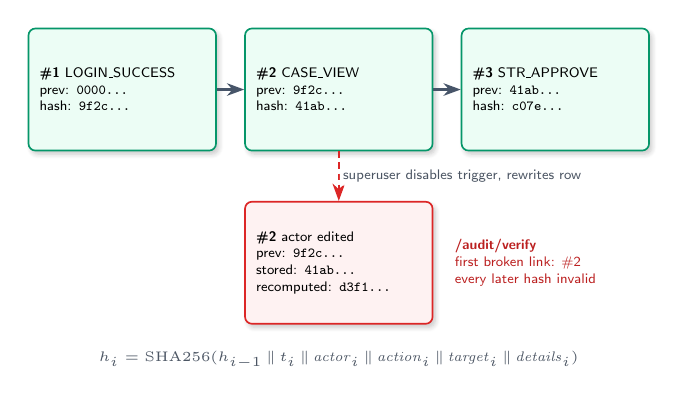
\begin{tikzpicture}[x=1cm,y=1cm,
  ent/.style={card, draw=dbS, fill=dbF, minimum width=2.25cm, minimum height=1.55cm, text width=2.1cm,
              font=\sffamily\tiny, align=left},
  bad/.style={card, draw=secS, fill=secF, minimum width=2.25cm, minimum height=1.55cm, text width=2.1cm,
              font=\sffamily\tiny, align=left}]
\node[ent] (e1) at (0,0)   {\textbf{\#1} LOGIN\_SUCCESS\\ prev: \texttt{0000\ldots}\\ hash: \texttt{9f2c\ldots}};
\node[ent] (e2) at (2.75,0) {\textbf{\#2} CASE\_VIEW\\ prev: \texttt{9f2c\ldots}\\ hash: \texttt{41ab\ldots}};
\node[ent] (e3) at (5.5,0) {\textbf{\#3} STR\_APPROVE\\ prev: \texttt{41ab\ldots}\\ hash: \texttt{c07e\ldots}};
\draw[arr] (e1) -- (e2); \draw[arr] (e2) -- (e3);

\node[bad] (t2) at (2.75,-2.2) {\textbf{\#2} actor edited\\ prev: \texttt{9f2c\ldots}\\ stored: \texttt{41ab\ldots}\\ recomputed: \texttt{d3f1\ldots}};
\draw[rdash, draw=secS] (e2) -- node[lbl, right] {superuser disables trigger, rewrites row} (t2);
\node[font=\sffamily\tiny, text=secS!85!black, align=left, anchor=west] at (4.1,-2.2)
  {\textbf{/audit/verify}\\first broken link: \#2\\every later hash invalid};
\node[font=\sffamily\tiny, text=inkM, anchor=north] at (2.75,-3.2)
  {$h_i = \mathrm{SHA256}(h_{i-1}\,\|\,t_i\,\|\,\mathit{actor}_i\,\|\,\mathit{action}_i\,\|\,\mathit{target}_i\,\|\,\mathit{details}_i)$};
\end{tikzpicture}
}
  \caption{Keyed hash chain. Rewriting entry \#2 invalidates its MAC and every later link; without
  the API's key, recomputing the chain does not help.}
  \label{fig:chain}
\end{figure}

Each entry stores $h_i = \mathrm{HMAC}_K(h_{i-1} \,\|\, t_i \,\|\, \mathit{actor}_i \,\|\,
\mathit{action}_i \,\|\, \mathit{target}_i \,\|\, \mathit{details}_i)$ (Fig.~\ref{fig:chain}).
Three layers protect it. A trigger blocks UPDATE, DELETE and TRUNCATE even for the superuser. A
superuser who disables the trigger and edits a row breaks the chain. One who also recomputes the
chain still fails, because the key $K$ is held only by the API process~\cite{schneier1999audit}. An
advisory lock serialises writers so concurrent requests cannot fork the chain. The residual risk is
an attacker who holds \emph{both} database access and the API key. Anchoring the chain head
periodically to write-once storage would close that gap.

% =====================================================================================
\section{Risk Management}\label{sec:risk}

\subsection{Method}\label{sec:method}
We follow the ISO~31000:2018 process~\cite{iso31000} (establish context, identify, analyse,
evaluate, treat, monitor), applied to information security as in ISO/IEC~27005:2022~\cite{iso27005},
with NIST SP~800-30's qualitative likelihood and impact scales~\cite{nist80030}. The system is
categorised by the RMF~\cite{nist80037} as \emph{high impact} for integrity, because a silenced alert
or forged STR has legal consequences, and \emph{moderate} for confidentiality and availability.

\subsection{Risk register}

\begin{table*}[t]
\caption{Risk register (5$\times$5; L = likelihood, I = impact, score = L$\times$I)}\label{tab:risk}
\centering\tbl
\begin{tabularx}{\textwidth}{@{}lp{3.4cm}cccLccc@{}}
\toprule
ID & Risk & L & I & Inherent & Treatment and controls & L & I & Residual \\ \midrule
R1 & Insider tampers with cases, alerts or audit trail & 4 & 5 & 20 & \textbf{Mitigate}: no-DELETE role, append-only trigger, keyed hash chain, maker--checker, evidence hashes & 2 & 5 & 10 \\
R2 & Analyst credentials compromised & 4 & 4 & 16 & \textbf{Mitigate}: bcrypt, short-lived JWT, RBAC, audited denials. \textbf{Gap}: no MFA or lockout & 3 & 4 & 12 \\
R3 & Disclosure of CNIC / phone numbers & 3 & 5 & 15 & \textbf{Mitigate}: masking, MLRO-only audited unmask, localhost binding. \textbf{Transfer}: cyber insurance (breach response) & 2 & 5 & 10 \\
R4 & Laundering goes undetected (regulatory penalty) & 5 & 4 & 20 & \textbf{Mitigate}: rules + graph + ML, look-alike testing, metrics. \textbf{Accept}: residual by senior management & 3 & 4 & 12 \\
R5 & Outage or data loss stops monitoring & 2 & 4 & 8 & \textbf{Mitigate}: health checks, restarts, idempotent replay. \textbf{Transfer}: business-interruption cover & 1 & 4 & 4 \\
R6 & Alert fatigue: true cases closed as false positives & 4 & 3 & 12 & \textbf{Mitigate}: case grouping, priority, explanations, closure reasons, SETA & 2 & 3 & 6 \\
\bottomrule
\end{tabularx}
\end{table*}

\begin{figure}[t]
  \centering
  \resizebox{0.95\columnwidth}{!}{% Risk heat map (Fig. 4): NIST SP 800-30 style 5x5, inherent -> residual.
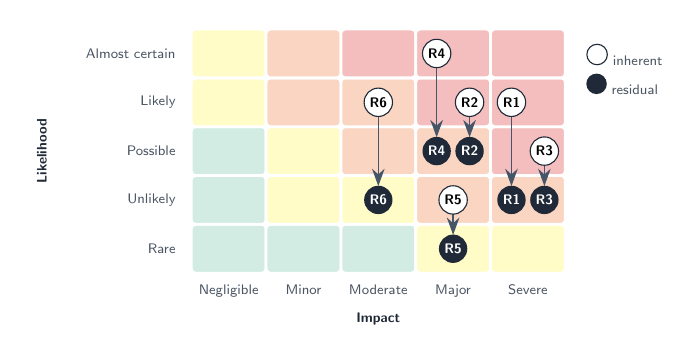
\begin{tikzpicture}[x=0.95cm,y=0.62cm, font=\sffamily\tiny]
\foreach \l in {1,...,5} \foreach \i in {1,...,5} {
  \pgfmathtruncatemacro{\sc}{\l*\i}
  \ifnum\sc>14 \def\c{secS!30}\else\ifnum\sc>7 \def\c{exS!25}\else\ifnum\sc>3 \def\c{yellow!22}\else\def\c{dbS!18}\fi\fi\fi
  \fill[\c, draw=white, line width=1pt, rounded corners=1.5pt] (\i-1,\l-1) rectangle (\i,\l);
}
\foreach \i/\t in {1/Negligible,2/Minor,3/Moderate,4/Major,5/Severe}
  \node[text=inkM, anchor=north] at (\i-0.5,-0.05) {\t};
\foreach \l/\t in {1/Rare,2/Unlikely,3/Possible,4/Likely,5/Almost certain}
  \node[text=inkM, anchor=east] at (-0.08,\l-0.5) {\t};
\node[text=inkD, font=\sffamily\bfseries\tiny] at (2.5,-0.95) {Impact};
\node[text=inkD, font=\sffamily\bfseries\tiny, rotate=90] at (-2.0,2.5) {Likelihood};
% inherent (hollow) -> residual (filled); coordinates = (impact-0.5, likelihood-0.5)
\foreach \id/\ix/\iy/\rx/\ry in {R1/4.28/3.5/4.28/1.5, R2/3.72/3.5/3.72/2.5, R3/4.72/2.5/4.72/1.5,
                                   R4/3.28/4.5/3.28/2.5, R5/3.5/1.5/3.5/0.5, R6/2.5/3.5/2.5/1.5} {
  \draw[->, draw=flow, line width=0.5pt, shorten >=5pt, shorten <=5pt] (\ix,\iy) -- (\rx,\ry);
  \node[circle, draw=inkD, fill=white, inner sep=0.5pt, minimum size=3.6mm, font=\sffamily\bfseries\tiny] at (\ix,\iy) {\id};
  \node[circle, fill=inkD, text=white, inner sep=0.5pt, minimum size=3.6mm, font=\sffamily\bfseries\tiny] at (\rx,\ry) {\id};
}
\node[anchor=north west, text=inkM, align=left] at (5.15,4.9)
  {\tikz\node[circle,draw=inkD,minimum size=2.6mm,inner sep=0]{};\ inherent\\[2pt]
   \tikz\node[circle,fill=inkD,minimum size=2.6mm,inner sep=0]{};\ residual};
\end{tikzpicture}
}
  \caption{Inherent $\rightarrow$ residual risk after the controls in Table~\ref{tab:risk}.}
  \label{fig:heat}
\end{figure}

Table~\ref{tab:risk} and Fig.~\ref{fig:heat} summarise the assessment. The highest residual risks
are R2, where multi-factor authentication is the clear next control, and R4, which no monitoring
system can drive to zero and which management must formally accept.

\subsection{Risk treatment and cyber insurance}
ISO~31000 offers four treatments: avoid, mitigate, transfer and accept. \emph{Transfer} through
cyber insurance suits risks whose financial impact can be estimated. Typical policies cover
first-party costs (forensics, notification, data restoration, business interruption) and
third-party liability for privacy breaches~\cite{marotta2017insurance}. Insurers increasingly price
policies by the controls in place, such as multi-factor authentication, logging, backups and an
incident-response plan~\cite{romanosky2019insurance}, so the controls in this project also lower
the premium.

Two limits matter for AML. First, regulatory fines and penalties for AML failures are commonly
excluded, or insurable only where law permits, so R4 cannot be transferred and must be mitigated and
accepted. Second, insurance pays for consequences but restores neither regulatory standing nor
customer trust. Insurance therefore complements controls and does not replace them.

\textbf{Illustrative quantification.} Following the annualised-loss approach in
Whitman and Mattord~\cite{whitman2012principles}, suppose a PII breach (R3) has a single loss
expectancy of PKR~25\,M and, before controls, an annual rate of occurrence of 0.3: the ALE is
PKR~7.5\,M. If masking and access control lower the rate to 0.05, the ALE falls to PKR~1.25\,M.
A policy priced below the remaining expected loss plus the cost of uncertainty is then a rational
transfer. These figures are illustrative assumptions, not market data.

% =====================================================================================
\section{Standards Compliance Mapping}

Table~\ref{tab:std} maps each implemented control to ISO/IEC~27001:2022 Annex~A~\cite{iso27001,iso27002},
NIST SP~800-53 Rev.~5~\cite{nist80053}, the CSF~2.0 categories~\cite{nistcsf2} and the relevant FATF
Recommendations~\cite{fatf2012rec}.

\begin{table*}[t]
\caption{Control mapping to standards}\label{tab:std}
\centering\tbl
\begin{tabularx}{\textwidth}{@{}Lllll@{}}
\toprule
WalletWatch control & ISO/IEC 27001:2022 Annex A & NIST SP 800-53 r5 & CSF 2.0 & FATF \\ \midrule
Transaction monitoring, typologies, ML scoring & 8.16 Monitoring activities & SI-4 & DE.CM, DE.AE & R.10, R.20 \\
STR workflow and goAML export & 5.31 Legal and regulatory requirements & AU-6 & GV.OC & R.20, R.21 \\
RBAC (analyst / mlro / auditor) & 5.15, 5.18, 8.3 & AC-2, AC-3 & PR.AA & --- \\
Maker--checker STR approval & 5.3 Segregation of duties & AC-5 & PR.AA & R.18 (internal controls) \\
Least-privilege DB roles; non-root containers & 8.2 Privileged access rights & AC-6, CM-7 & PR.AA, PR.PS & --- \\
bcrypt + JWT authentication & 5.17, 8.5 Secure authentication & IA-2, IA-5 & PR.AA & --- \\
PII masking, audited unmask & 8.11 Data masking; 5.34 PII protection & AC-3, SI-19 & PR.DS & R.21 (confidentiality) \\
Keyed hash-chained audit log & 8.15 Logging; 5.33 Protection of records & AU-2, AU-3, AU-9(3), AU-10 & DE.CM, PR.PS & R.11 (records) \\
Evidence hashing; DB constraints & 8.28 Secure coding & SI-7, SI-10 & PR.DS & R.11 \\
Automated security tests & 8.29 Security testing & SA-11, CA-2 & ID.IM & --- \\
Health checks, restart, idempotent replay & 8.14 Redundancy & CP-10 & PR.IR, RC.RP & --- \\
SETA programme (Section~\ref{sec:seta}) & 6.3 Awareness, education, training & AT-2, AT-3 & PR.AT & R.18 \\
Risk assessment (Section~\ref{sec:risk}) & Clauses 6.1.2, 8.2 & RA-3 & ID.RA, GV.RM & R.1 (risk-based approach) \\
\bottomrule
\end{tabularx}
\end{table*}

\textbf{RMF view.} Following the RMF, the project was categorised (Section~\ref{sec:method}); controls were
selected and implemented (Sections~\ref{sec:arch}--\ref{sec:ia}), assessed by the automated suite, and are monitored
continuously through the evaluator and the audit verification endpoint. Authorisation to operate
remains an organisational decision outside the project.

\textbf{Known gaps.} The project does not implement multi-factor authentication (IA-2(1)),
encryption at rest for PII (SC-28), TLS in transit (SC-8) or account lockout (AC-7). Each is listed
as future work and reflected in the residual risks.

% =====================================================================================
\section{Security Education, Training and Awareness}\label{sec:seta}

Technology controls fail when people misuse them. An analyst who closes alerts without reading
them, or an MLRO who shares a password, defeats maker--checker. Whitman and Mattord's SETA model
distinguishes \emph{awareness} (what), \emph{training} (how) and \emph{education}
(why)~\cite{whitman2012principles}. NIST SP~800-50 Rev.~1 describes how to build such a learning
programme around roles~\cite{nist80050r1}. Table~\ref{tab:seta} gives a programme for a wallet
operator running WalletWatch.

\begin{table*}[t]
\caption{SETA programme for WalletWatch users}\label{tab:seta}
\centering\tbl
\begin{tabularx}{\textwidth}{@{}p{1.25cm}p{2.0cm}Xp{3.6cm}p{3.4cm}@{}}
\toprule
Layer & Audience & Content & Delivery / frequency & Effectiveness measure \\ \midrule
Awareness & All staff, agents & What laundering looks like at a counter; red flags (structuring, one person with many wallets); how to report internally; never tip off a customer (AMLA 2010, FATF R.21) & e-learning at onboarding + yearly; posters at agent outlets & completion rate; internal reports per agent \\
Awareness & Customers & Never share PIN or OTP; don't lend your wallet; mule recruitment scams & SMS / in-app campaigns, quarterly & reported scam attempts \\
Training & Analysts & The six typologies; reading evidence and SHAP; writing closure reasons; evidence integrity; data-handling rules & hands-on lab with WalletWatch's synthetic data; before access, then semi-annual & QA sample of closed cases; FP-closure accuracy vs ground truth \\
Training & MLROs & STR quality and narrative; maker--checker responsibilities; justified unmasking; goAML submission & workshop + shadowing; yearly & STR rejection rate by FMU; audit of unmask reasons \\
Training & Auditors, admins & Verifying the audit chain; access reviews; key and secret handling & runbook drills; semi-annual & time to detect a planted tamper \\
Education & Compliance and security leads & AML law and FATF standards; risk management; secure system design & certifications (e.g.\ CAMS, CISSP), university courses & certifications held; audit findings \\
\bottomrule
\end{tabularx}
\end{table*}

The system supports SETA directly. Its synthetic world doubles as a safe training range where
analysts practise on realistic cases without touching real customer data. Because ground truth is
known, an analyst's closure decisions can be scored. SHAP explanations and evidence views teach
\emph{why} a pattern is suspicious, and the tamper demonstration makes the value of the audit trail
concrete for auditors.

% =====================================================================================
\section{Evaluation}

\subsection{Machine-learning model (offline)}
On the held-out world (seed 13, \ResMLTestTxns\ transactions, \ResMLTestIllicit\ illicit) the model
reaches PR-AUC~\ResMLPRAUC\ and ROC-AUC~\ResMLROC. At the operating threshold of 0.80, precision is
\ResMLPrec\ and recall \ResMLRec. PR-AUC is the meaningful figure at this level of imbalance. The
model flags \ResMLCommittee\ of committee payments, a genuine, explainable false-positive mode.

\subsection{Live run}
The simulator streamed \ResTxns\ transactions over \ResDays\ simulated days (seed 42) through the
full system. Tables~\ref{tab:live} and~\ref{tab:typo} give account-level results from the evaluator:
an alerted account is a true positive if it belongs to a laundering ring.

% Generated by scripts/export_results.py — do not edit.
\begin{table}[!t]
\caption{Live run: accounts alerted per scenario}\label{tab:live}
\centering\tbl
\begin{tabularx}{\columnwidth}{@{}llrrrrr@{}}
\toprule
ID & Scenario & Alerted & TP & Look-alike & Other & Prec. \\ \midrule
ML & Model risk & 152 & 47 & 3 & 102 & 31\% \\
S1 & Structuring & 11 & 7 & 0 & 4 & 64\% \\
S2 & Fan-in/out mule & 2 & 2 & 0 & 0 & 100\% \\
S3 & Pass-through & 17 & 14 & 0 & 3 & 82\% \\
S4 & Layering chain & 15 & 15 & 0 & 0 & 100\% \\
S5 & Round-trip & 13 & 10 & 0 & 3 & 77\% \\
S6 & Shared device & 37 & 7 & 30 & 0 & 19\% \\
\midrule
\multicolumn{2}{@{}l}{All scenarios (distinct accounts)} & 192 & 47 & \multicolumn{2}{c}{} & 24\% \\
\bottomrule
\end{tabularx}
\end{table}

\begin{table}[!t]
\caption{Live run: recall by typology, time to detect, look-alikes}\label{tab:typo}
\centering\tbl
\begin{tabularx}{\columnwidth}{@{}Xrrr@{}}
\toprule
Typology & Active accounts & Recall (rules) & Recall (+ML) \\ \midrule
Structuring & 9 & 78\% & 100\% \\
Fan-in/out mule & 15 & 13\% & 67\% \\
Pass-through & 6 & 33\% & 50\% \\
Layering chain & 16 & 94\% & 94\% \\
Round-trip & 10 & 100\% & 100\% \\
\midrule
\multicolumn{3}{@{}l}{Overall recall, active illicit accounts (56)} & 84\% \\
\bottomrule
\end{tabularx}\\[6pt]
\begin{tabularx}{\columnwidth}{@{}Xrrr@{}}
\toprule
Typology & Rings detected & Fastest (h) & Slowest (h) \\ \midrule
Structuring & 2 & 0.0 & 0.0 \\
Fan-in/out mule & 2 & 5.4 & 5.7 \\
Pass-through & 2 & 0.0 & 0.7 \\
Layering chain & 2 & 0.0 & 0.6 \\
Round-trip & 2 & 0.0 & 0.0 \\
\bottomrule
\end{tabularx}\\[6pt]
\begin{tabularx}{\columnwidth}{@{}Xrr@{}}
\toprule
Benign look-alike & Accounts & Alerted \\ \midrule
Committee organisers & 8 & 3 \\
Family chain members & 90 & 0 \\
Salary employers & 5 & 0 \\
Shared-phone wallets & 30 & 30 \\
\bottomrule
\end{tabularx}
\end{table}


\textbf{Discussion.} The graph scenarios (S4, S5) are precise, because chains and cycles of
near-equal amounts are rare in normal behaviour. The device rule (S6) is the noisiest by design:
shared family phones trigger it, and the analyst closes those cases with a reason. Rules alone miss
most downstream mules in fan-out rings, because each receives only one payment before cashing out.
The model recovers part of them, which shows the value of the hybrid design. Time to detect is
measured from a ring's first illicit transaction to the first alert on any member.

\subsection{Performance}
On a laptop the API sustains about 100 transactions per second with all rules and ML scoring.
That is about three times the average rate the live demo needs, and each graph-worker tick completes in under a
second.

% =====================================================================================
\section{Limitations and Future Work}
The data is synthetic and the rules were designed alongside the simulator, so the scores are
optimistic. Look-alikes, a held-out seed for the model, and reporting false positives openly reduce
this circularity but do not remove it. Tier limits are illustrative, and the CTR threshold is
documented but not implemented. Production use would need TLS, single sign-on with MFA, encryption
at rest with managed keys, an externally anchored audit head, rule back-testing, a feedback loop
that retrains on analyst decisions, sanctions screening and goAML XML export.

% =====================================================================================
\section{Conclusion}
WalletWatch shows that an AML monitoring system can be built as a security system and not only as
a detector. Its detection combines explainable rules, temporal graph analysis and an explained
model, and is evaluated honestly against benign look-alikes. Its assurance rests on controls drawn
from ISO/IEC 27001, NIST SP 800-53 and FATF, on a documented risk treatment that includes cyber
insurance, on a SETA programme for its users, and on an automated test for every security claim.

\balance
\bibliographystyle{ieeetr}
\bibliography{refs}

\end{document}
